\chapter{सतत रिएक्टर और औद्योगिक प्रक्रम}\label{ch:b2:continuous-reactors}

प्रयोगशाला में अभिक्रिया फ़्लास्क में की जाती है: अभिकर्मक डाले जाते हैं,
मिश्रण को एक घंटे विलोडित किया जाता है, अभिक्रिया रोकी जाती है और उत्पाद
पृथक किया जाता है। वही उत्पाद हज़ारों टन में बनाने वाला संयंत्र भिन्न
ढंग से काम करता है। उसका रिएक्टर कभी खाली नहीं होता: एक सिरे से अभिकारक भीतर बहते हैं,
दूसरे से उत्पाद बाहर, दिन-रात, और भीतर का संघटन
समय के साथ नहीं बदलता। तब ``कितनी देर?'' के स्थान पर दो प्रश्न आते हैं: किसी दिए गए
\omterm{def:b2:continuous-reactors:conversion}{रूपांतरण} के लिए रिएक्टर कितना बड़ा हो, और अभिक्रिया की ऊष्मा को, रिएक्टर को
बेकाबू गर्म करने से पहले, कैसे हटाया जाए? यह अध्याय दो आदर्श \omterm{def:b2:continuous-reactors:reactors}{सतत रिएक्टरों},
विलोडित टंकी और नली, के लिए द्रव्य और ऊर्जा के संतुलन लिखता है, उनकी तुलना करता है, और
दिखाता है कि किसी रिएक्टर की कई संभव अवस्थाएँ हो सकती हैं, जिनमें से एक
अनियंत्रण है।

\begin{recall}
प्रथम वर्ष का खंड: अभिक्रिया की दर, दर नियम और कोटियाँ, बंद रिएक्टर (जिसे अब
\omterm{def:b2:continuous-reactors:reactors}{बैच रिएक्टर} कहा जाता है) के समाकलित नियम, अर्ध-आयु, आरेनियस
नियम $k = A\,\mathrm e^{-E_a/RT}$, क्रमागत अभिक्रियाएँ।
\Cref{ch:b2:reaction-enthalpy}: नियत दाब पर मुक्त ऊष्मा;
\cref{ch:b2:equilibrium-shifts}: \omterm{def:b2:equilibrium-shifts:single-pass}{एकल-पारण रूपांतरण}, \omterm{def:b2:equilibrium-shifts:single-pass}{पुनश्चक्रण}। भौतिकी से:
स्थायी प्रवाह में खुले निकाय का संतुलन (जो प्रवेश करता है ऋण
जो निकलता है बराबर जो संचित होता है)।
\end{recall}

\begin{omfigure}
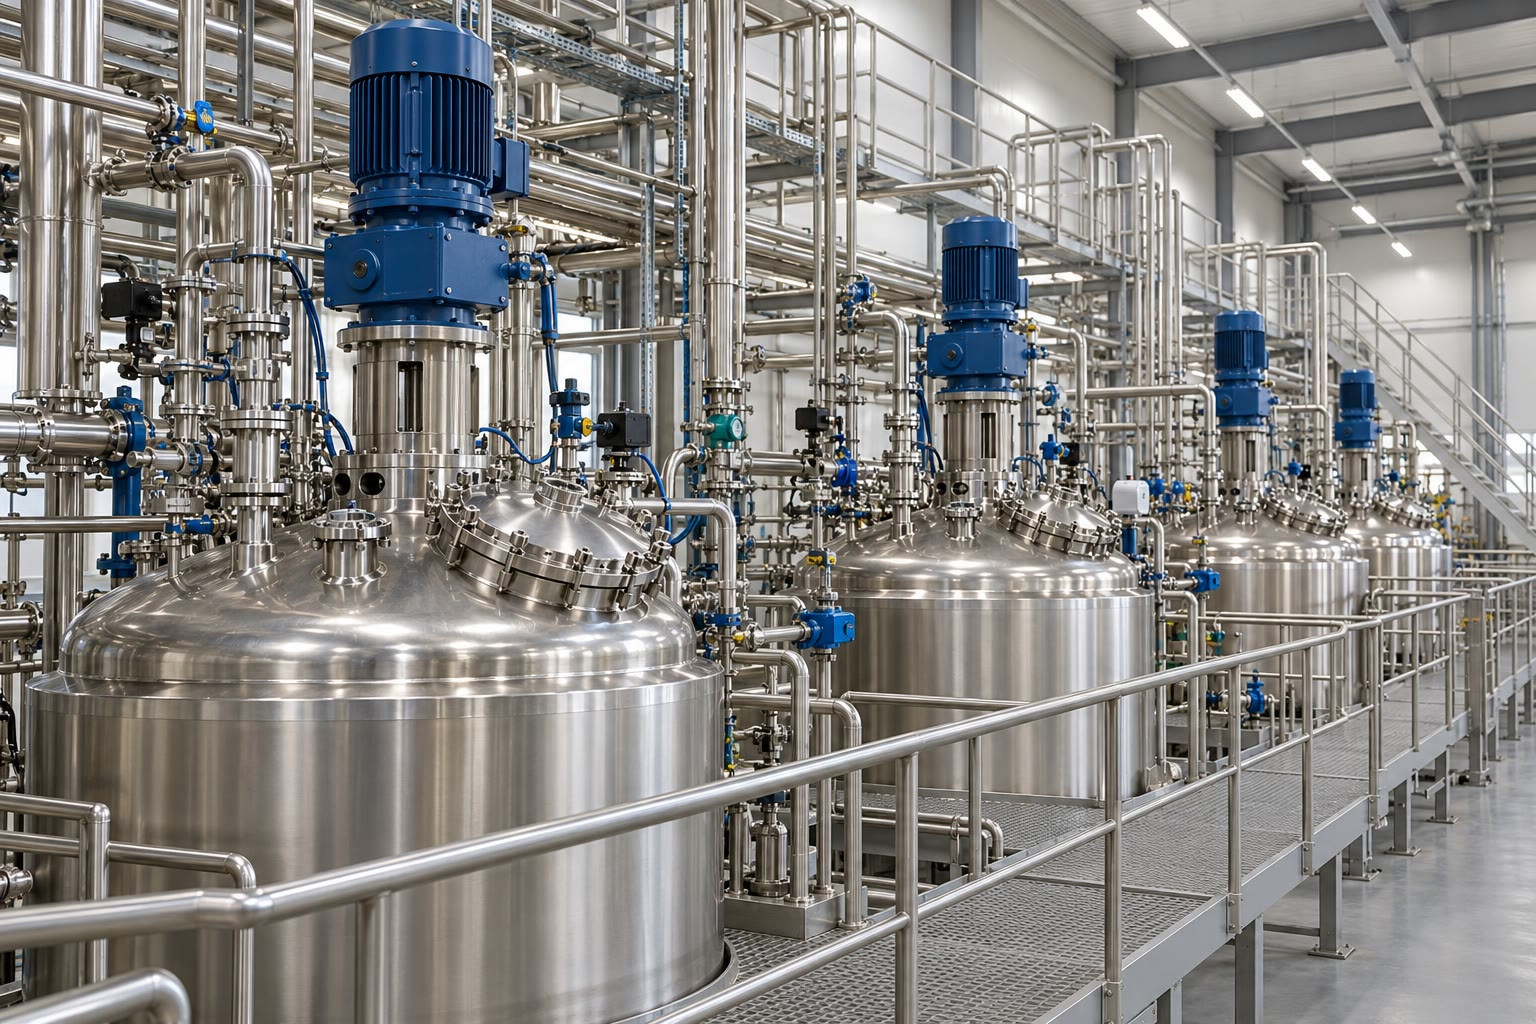
\includegraphics[width=0.6\linewidth]{images/book3/ai/b2-05-stirred-tanks.jpg}

{\small किसी रासायनिक संयंत्र में विलोडित-टंकी रिएक्टर: हर पात्र पर उसकी
मोटर और गियरबॉक्स है, विलोडक का शाफ़्ट अभिक्रिया-मिश्रण में नीचे जाता है;
पाइप फ़ीड लाते हैं और उत्पाद तथा शीतलन जल ले जाते हैं।}
\end{omfigure}

\section{बैच से सतत तक}

\begin{definition}[रिएक्टर के प्रकार]\label{def:b2:continuous-reactors:reactors}
\emph{बैच रिएक्टर}\index{बैच रिएक्टर} एक बंद पात्र है जिसमें
द्रव्य के अंतर्वाह या बहिर्वाह के बिना अभिक्रिया होती है।
\emph{सतत रिएक्टर}\index{सतत रिएक्टर} से होकर द्रव्य का स्थायी
प्रवाह गुज़रता है। दो आदर्श सतत रिएक्टर मॉडल का काम करते हैं:
\begin{itemize}
  \item \emph{सतत विलोडित-टंकी रिएक्टर}\index{सतत विलोडित-टंकी रिएक्टर}
(CSTR), इतना अच्छी तरह विलोडित कि उसकी अंतर्वस्तु
        एकसमान है, और इसलिए उससे निकलने वाली धारा के सर्वसम है;
  \item \emph{प्लग-प्रवाह रिएक्टर}\index{प्लग-प्रवाह रिएक्टर} (PFR), एक नली
        जिससे तरल प्रवाह की दिशा में बिना मिश्रण के गुज़रता है, तरल का हर
        खंड अभिक्रिया करते हुए पिस्टन की तरह आगे बढ़ता है।
\end{itemize}
\end{definition}

कोई \omterm{def:b2:continuous-reactors:reactors}{सतत रिएक्टर} \emph{स्थायी संचालन} में कहलाता है जब उसके भीतर
कुछ भी समय के साथ नहीं बदलता: हर बिंदु पर प्रवाह, ताप और
संघटन स्थिर रहते हैं। हम एक ही अभिक्रिया
$\mathrm A \to$ उत्पाद लेते हैं, स्थिर घनत्व का द्रव फ़ीड (जिससे
आयतनी प्रवाह दर $Q_v$ प्रवेश और निकास पर समान है), जिसकी प्रवेश पर
सांद्रता $c_{A,0}$ है।

\begin{definition}[निवास काल]\label{def:b2:continuous-reactors:residence-time}
आयतन $V$ वाले और आयतनी प्रवाह दर $Q_v$ पर पोषित \omterm{def:b2:continuous-reactors:reactors}{सतत रिएक्टर} का
\emph{निवास काल}\index{निवास काल} $\tau = V/Q_v$ है: वह माध्य
समय जो तरल का कोई आयतन उसके भीतर बिताता है।
\end{definition}

\begin{definition}[रूपांतरण]\label{def:b2:continuous-reactors:conversion}
अभिकारक A का \emph{रूपांतरण}\index{रूपांतरण} $X = (F_{A,0} -
F_A)/F_{A,0}$ है, जहाँ $F_{A,0}$ और $F_A$, A की रिएक्टर में प्रवेश करने और
उससे निकलने वाली मोलर प्रवाह दरें हैं; \omterm{def:b2:continuous-reactors:reactors}{बैच रिएक्टर} के लिए $X = (n_{A,0} -
n_A)/n_{A,0}$। स्थिर घनत्व पर $X = 1 - c_A/c_{A,0}$।
\end{definition}

\omterm{def:b2:continuous-reactors:conversion}{रूपांतरण} एक अभिकारक का, और किसी रिएक्टर या पारण का होता है; प्रथम वर्ष के खंड की
अंतिम आंशिक प्रगति किसी अभिक्रिया और उसके सीमांत अभिकारक की होती है।
एक ही अभिक्रिया के लिए जिसका सीमांत अभिकारक A है, दोनों
संपाती होते हैं।

\begin{proposition}[बैच रिएक्टर]\label{prop:b2:continuous-reactors:batch}
नियत आयतन के \omterm{def:b2:continuous-reactors:reactors}{बैच रिएक्टर} में प्रथम कोटि की अभिक्रिया \omterm{def:b2:continuous-reactors:conversion}{रूपांतरण}
$X = 1 - \mathrm e^{-kt}$ तक समय $t$ के बाद पहुँचती है, और समान प्रारंभिक
सांद्रताओं $c_0$ वाली द्वितीय कोटि की अभिक्रिया \omterm{def:b2:continuous-reactors:conversion}{रूपांतरण} $X =
kc_0t/(1 + kc_0t)$ तक।
\end{proposition}

\begin{proof}
ये प्रथम वर्ष के खंड के समाकलित दर नियम हैं, $c_A = c_{A,0}
\mathrm e^{-kt}$ और $1/c_A = 1/c_{A,0} + kt$, जिन्हें $X = 1 -
c_A/c_{A,0}$ के साथ लिखा गया है।
\end{proof}

\section{सतत विलोडित-टंकी रिएक्टर}

\begin{omfigure}
\begin{tikzpicture}[font=\small, >={Stealth}]
  % batch
  \pic[transform shape] at (0,0) {rbflask={0.6}{omDef!20}};
  \node[below] at (0,-0.15) {बैच};
  % CSTR
  \begin{scope}[xshift=4.2cm]
    \draw[thick, fill=omDef!15] (-1.2,0) rectangle (1.2,2.4);
    \draw[thick] (0,3.0) -- (0,0.5);
    \draw[thick, fill=gray!40] (-0.5,0.45) rectangle (0.5,0.6);
    \draw[thick, fill=gray!30] (-0.25,3.0) rectangle (0.25,3.35);
    \draw[->, thick, omDef] (-2.8,2.0) -- (-1.2,2.0) node[pos=0.0, above, anchor=south west, inner sep=1pt] {$Q_v$, $c_{A,0}$};
    \draw[->, thick, omThm] (1.2,0.3) -- (2.5,0.3) node[pos=1, below] {$Q_v$, $c_A$};
    \node[fill=omDef!15, inner sep=1pt] at (0.62,1.5) {$V$, $c_A$};
    \node[below] at (0,-0.15) {विलोडित टंकी};
  \end{scope}
  % PFR
  \begin{scope}[xshift=8.4cm, yshift=1.0cm]
    \draw[thick, fill=omDef!10] (0,0) rectangle (4.2,0.7);
    \fill[omThm!25] (2.0,0) rectangle (2.35,0.7);
    \draw[thick] (2.0,0) -- (2.0,0.7) (2.35,0) -- (2.35,0.7);
    \node[above] at (2.17,0.75) {$\dd V$};
    \draw[->, thick, omDef] (-0.9,0.35) -- (0,0.35) node[pos=0, above] {$F_{A,0}$};
    \draw[->, thick, omThm] (4.2,0.35) -- (5.0,0.35) node[pos=1, above] {$F_A$};
    \node[below] at (1.0,0) {$F_A(V)$};
    \node[below] at (2.1,-1.15) {प्लग-प्रवाह नली};
  \end{scope}
\end{tikzpicture}

{\small तीन आदर्श रिएक्टर। एक बैच फ़्लास्क; एक विलोडित टंकी जिसकी एकसमान
अंतर्वस्तु निकास धारा जैसी है; प्लग प्रवाह में तय की जाने वाली एक नली, जिसमें
A की प्रवाह दर खंड-दर-खंड घटती है।}
\end{omfigure}

\begin{proposition}[विलोडित टंकी का संतुलन]\label{prop:b2:continuous-reactors:cstr-balance}
स्थायी संचालन में, आयतन $V$ की विलोडित टंकी, जिसमें A दर $r$ (mol प्रति
लीटर और प्रति सेकंड) से लुप्त होता है, यह संतुष्ट करती है:
\[
  F_{A,0} - F_A - rV = 0, \qquad\text{अर्थात्}\qquad c_{A,0} - c_A = r\,\tau ,
\]
जहाँ दर निकास के संघटन और ताप पर ली जाती है।
\end{proposition}

\begin{proof}
समय $\dd t$ में टंकी पर A का संतुलन: जो प्रवेश करता है, $F_{A,0}\dd t$,
ऋण जो निकलता है, $F_A\dd t$, ऋण जो अभिक्रिया करता है, $rV\dd t$, बराबर
संचय, जो स्थायी संचालन में शून्य है। टंकी एकसमान है, इसलिए दर
हर जगह समान है और निकास धारा की दर के बराबर है। $Q_v$ से भाग दीजिए।
\end{proof}

\begin{theorem}[विलोडित टंकी में रूपांतरण]\label{thm:b2:continuous-reactors:cstr}
प्रथम कोटि की अभिक्रिया के लिए $X = \dfrac{k\tau}{1 + k\tau}$; दोनों
अभिकारकों की समान फ़ीड सांद्रताओं $c_0$ वाली द्वितीय कोटि की अभिक्रिया के लिए
$X$ अंतराल $[0, 1]$ में स्थित वह मूल है जो $Da\,(1 - X)^2 = X$ का है, जहाँ $Da =
kc_0\tau$।
\end{theorem}

\begin{proof}
कोटि 1: $r = kc_A$, अतः $c_{A,0} - c_A = k\tau c_A$, $c_A = c_{A,0}/(1 + k\tau)$
और $X = 1 - 1/(1 + k\tau)$। कोटि 2: $r = kc_A^2$ (दोनों सांद्रताएँ
समान रहती हैं), $c_0X = k\tau c_0^2(1 - X)^2$।
\end{proof}

विमाहीन समूह $Da = k\tau$ (या $kc_0\tau$), डाम्कोलर
संख्या, \omterm{def:b2:continuous-reactors:residence-time}{निवास काल} की तुलना अभिक्रिया के समय-पैमाने से करती है:
केवल वही \omterm{def:b2:continuous-reactors:conversion}{रूपांतरण} तय करती है।

\begin{method}[रिएक्टर का आकार तय करना]\label{met:b2:continuous-reactors:size-reactor}
\begin{enumerate}
  \item दर नियम और आवश्यक \omterm{def:b2:continuous-reactors:conversion}{रूपांतरण} $X$ लिखिए।
  \item चुने गए रिएक्टर के संतुलन से वह डाम्कोलर संख्या ज्ञात कीजिए
        जो $X$ देती है।
  \item $\tau$ को $Da$ और कार्य-ताप पर दर स्थिरांक से निकालिए,
        और उपचारित किए जाने वाले प्रवाह से $V = \tau Q_v$।
\end{enumerate}
\end{method}

\section{प्लग-प्रवाह रिएक्टर}

\begin{theorem}[प्लग-प्रवाह रिएक्टर में रूपांतरण]\label{thm:b2:continuous-reactors:pfr}
स्थायी संचालन में प्लग-प्रवाह नली के अनुदिश A की प्रवाह दर
$\dd F_A/\dd V = -r$ का पालन करती है। प्रथम कोटि की अभिक्रिया के लिए इससे $X = 1 -
\mathrm e^{-k\tau}$ मिलता है, और समान फ़ीड वाली द्वितीय कोटि की अभिक्रिया के लिए $X =
Da/(1 + Da)$: ये \omterm{def:b2:continuous-reactors:reactors}{बैच रिएक्टर} के नियम हैं, समय के स्थान पर
\omterm{def:b2:continuous-reactors:residence-time}{निवास काल} के साथ।
\end{theorem}

\begin{proof}
$V$ और $V + \dd V$ के बीच के खंड पर A का संतुलन: $F_A(V) - F_A(V + \dd V)
- r\,\dd V = 0$, अतः अवकल समीकरण। $F_A = Q_vc_A$ और
$\dd V = Q_v\,\dd t'$ (वह समय $t'$ जो किसी खंड ने नली में बिताया है) के साथ यह
$\dd c_A/\dd t' = -r$ बनता है: हर खंड एक छोटा \omterm{def:b2:continuous-reactors:reactors}{बैच रिएक्टर} है जो
नली में $\tau$ समय तक रहता है। $r = kc_A$ के लिए चरों को पृथक करने पर निकास पर $c_A = c_{A,0}
\mathrm e^{-k\tau}$ मिलता है; $r = kc_A^2$ के लिए $1/c_A - 1/c_0 = k\tau$।
\end{proof}

\begin{omfigure}
\begin{tikzpicture}
\begin{axis}[
  width=0.75\linewidth, height=6cm, xmin=0, xmax=10, ymin=0, ymax=1.05,
  axis x line=bottom, axis y line=left, xlabel={डाम्कोलर संख्या $k\tau$},
  ylabel={रूपांतरण $X$}, tick label style={font=\small},
  label style={font=\small}, clip=false,
  legend style={font=\scriptsize, draw=none, at={(0.98,0.05)}, anchor=south east}]
\addplot[omThm, very thick] table[x=Da, y=pfr] {figdata/out/bachelor-2-reactors-a.dat};
\addplot[omProp, thick] table[x=Da, y=five] {figdata/out/bachelor-2-reactors-a.dat};
\addplot[omProp, thick, dashed] table[x=Da, y=two] {figdata/out/bachelor-2-reactors-a.dat};
\addplot[omDef, very thick] table[x=Da, y=cstr] {figdata/out/bachelor-2-reactors-a.dat};
\legend{प्लग प्रवाह, श्रेणी में 5 टंकियाँ, श्रेणी में 2 टंकियाँ, 1 विलोडित टंकी}
\draw[dotted] (axis cs:2.303,0) -- (axis cs:2.303,0.9) -- (axis cs:9,0.9);
\fill[omThm] (axis cs:2.303,0.9) circle (1.4pt);
\fill[omDef] (axis cs:9,0.9) circle (1.4pt);
\end{axis}
\end{tikzpicture}

{\small आदर्श रिएक्टरों में $k\tau$ के सापेक्ष प्रथम कोटि की अभिक्रिया का
\omterm{def:b2:continuous-reactors:conversion}{रूपांतरण}। 90\,\% \omterm{def:b2:continuous-reactors:conversion}{रूपांतरण} के लिए प्लग-प्रवाह नली को $k\tau = \ln 10 = 2.3$ चाहिए,
एक अकेली विलोडित टंकी को $k\tau = 9$: चार गुना आयतन। श्रेणी में टंकियाँ
नली के निकट पहुँचती हैं।}
% (model curves, computed in figdata/bachelor-2/reactors.py)
\end{omfigure}

\begin{proposition}[टंकी या नली]\label{prop:b2:continuous-reactors:compare}
A की सांद्रता के साथ बढ़ने वाली किसी भी दर (कोई भी धनात्मक
कोटि) के लिए, \omterm{def:b2:continuous-reactors:reactors}{प्लग-प्रवाह रिएक्टर} दिए गए \omterm{def:b2:continuous-reactors:conversion}{रूपांतरण} तक विलोडित टंकी की तुलना में
छोटे आयतन से पहुँचता है।
\end{proposition}

\begin{proof}
संतुलनों से $\tau_{\text{CSTR}} = c_{A,0}X/r(X)$ (निकास
संघटन पर दर) और $\tau_{\text{PFR}} = c_{A,0}\int_0^X\dd X'/r(X')$। चूँकि $r$
घटता है जब $X$ बढ़ता है, $1/r(X') \leq 1/r(X)$ अंतराल $[0, X]$ पर, अतः
समाकल अधिकतम $X/r(X)$ है। आलेखीय रूप से, $1/r$ को $X$ के सापेक्ष दर्शाने वाले चार्ट पर
नली का $\tau$ वक्र के नीचे का क्षेत्रफल है और टंकी का \omterm{def:b2:continuous-reactors:residence-time}{निवास काल}
ऊँचाई $1/r(X)$ वाला आयत (नीचे का चित्र)। कोटि 1 के लिए: $\ln(1 + k\tau) \leq k\tau$, जो
दूसरे रूप में वही कथन है।
\end{proof}

विलोडित टंकी पूरी तरह निकास सांद्रता पर, जो निकाय में सबसे कम है,
और इसलिए सबसे कम दर पर काम करती है; नली अपने प्रवेश के निकट की उच्च
सांद्रताओं का उपयोग करती है। टंकी के लाभ कहीं और हैं: एकसमान, आसानी से
नियंत्रित ताप, और सरल संचालन।

\begin{omfigure}
\begin{tikzpicture}
\begin{axis}[
  width=0.62\linewidth, height=5.6cm, xmin=0, xmax=1, ymin=0, ymax=22,
  axis x line=bottom, axis y line=left, xlabel={रूपांतरण $X$},
  ylabel={$1/r$ (मॉडल इकाइयाँ)}, tick label style={font=\small},
  label style={font=\small}, clip=false]
\fill[omDef!15] (axis cs:0,0) rectangle (axis cs:0.9,10);
\addplot[omThm, fill=omThm!20, draw=none, domain=0:0.9, samples=60] {1/(1-x)} \closedcycle;
\addplot[black, very thick] table[x=X, y=invr] {figdata/out/bachelor-2-reactors-c.dat};
\draw[omDef, thick] (axis cs:0,10) -- (axis cs:0.9,10) -- (axis cs:0.9,0);
\node[omDef, font=\scriptsize, anchor=south] at (axis cs:0.45,10.2) {विलोडित टंकी: आयत, $\tau = 9$};
\node[omThm, font=\scriptsize, anchor=west] (pf) at (axis cs:0.05,6.5) {प्लग प्रवाह: छायांकित क्षेत्र, $\tau = \ln 10$};
\draw[omThm, ->] (axis cs:0.25,6.0) -- (axis cs:0.3,0.8);
\end{axis}
\end{tikzpicture}

{\small प्रथम कोटि की अभिक्रिया का लेवेनस्पील आलेख ($k = 1$, $c_{A,0} = 1$)।
90\,\% \omterm{def:b2:continuous-reactors:conversion}{रूपांतरण} के लिए विलोडित टंकी को पूरा आयत चाहिए, प्लग
प्रवाह को केवल वक्र के नीचे का छायांकित क्षेत्र।}
% (model, computed in figdata/bachelor-2/reactors.py)
\end{omfigure}

\begin{proposition}[श्रेणी में टंकियाँ]\label{prop:b2:continuous-reactors:cascade}
श्रेणी में $N$ समान विलोडित टंकियाँ, कुल \omterm{def:b2:continuous-reactors:residence-time}{निवास काल} $\tau$ के साथ,
प्रथम कोटि की अभिक्रिया को $X_N = 1 - (1 + k\tau/N)^{-N}$ तक रूपांतरित करती हैं, जो
$N$ के साथ बढ़ता है और प्लग-प्रवाह मान $1 - \mathrm e^{-k\tau}$ की ओर प्रवृत्त होता है।
\end{proposition}

\begin{proof}
हर टंकी सांद्रता को $1 + k\tau/N$ से भाग देती है। और $(1 +
k\tau/N)^{-N} = \exp[-N\ln(1 + k\tau/N)] \to \mathrm e^{-k\tau}$, क्योंकि
$N\ln(1 + u/N) \to u$।
\end{proof}

\begin{definition}[वरणात्मकता]\label{def:b2:continuous-reactors:selectivity}
जब कोई अभिकारक कई उत्पाद दे सकता है, तो वांछित उत्पाद B के लिए
\emph{वरणात्मकता}\index{वरणात्मकता} बने B की मात्रा को उपभुक्त
अभिकारक की मात्रा से भाग देने पर (रससमीकरणमितीय अनुपात से गुणा करके) मिलती है: यह बताती है कि
जो अभिक्रिया हुई उसका कितना भाग सही दिशा में गया।
\end{definition}

\begin{proposition}[टंकी और नली में एक मध्यवर्ती]\label{prop:b2:continuous-reactors:consecutive}
क्रमागत प्रथम कोटि अभिक्रियाओं $\mathrm A \xrightarrow{k_1} \mathrm B
\xrightarrow{k_2} \mathrm C$ के लिए, केवल A वाले फ़ीड के साथ, निकास पर B की
सांद्रता \omterm{def:b2:continuous-reactors:reactors}{प्लग-प्रवाह रिएक्टर} में $\tau = \ln(k_2/k_1)/(k_2 - k_1)$ पर
और विलोडित टंकी में $\tau = 1/\sqrt{k_1k_2}$ पर अधिकतम होती है;
नली में अधिकतम मान ऊँचा होता है।
\end{proposition}

\begin{proof}
नली: प्रथम वर्ष के खंड के बैच नियम, $c_B = c_{A,0}\frac{k_1}{k_2 - k_1}
(\mathrm e^{-k_1\tau} - \mathrm e^{-k_2\tau})$, अधिकतम वहाँ जहाँ अवकलज
शून्य हो, $k_1\mathrm e^{-k_1\tau} = k_2\mathrm e^{-k_2\tau}$। टंकी: $c_A =
c_{A,0}/(1 + k_1\tau)$ और B का संतुलन, $c_B = k_1\tau c_A - k_2\tau c_B$,
$c_B = c_{A,0}k_1\tau/[(1 + k_1\tau)(1 + k_2\tau)]$ देता है, जिसका अवकलज
$k_1k_2\tau^2 = 1$ होने पर शून्य होता है। अधिकतम मानों की तुलना
\cref{exo:b2:continuous-reactors:10} है।
\end{proof}

\section{ऊष्मा संतुलन और सुरक्षा}

\begin{definition}[रुद्धोष्म ताप-वृद्धि]\label{def:b2:continuous-reactors:adiabatic-rise}
किसी अभिक्रिया-मिश्रण की \emph{रुद्धोष्म ताप-वृद्धि}\index{रुद्धोष्म ताप-वृद्धि}
$\Delta T_{\text{ad}}$ ताप की वह वृद्धि है जो उसमें होती यदि
अभिक्रिया पूर्ण होती और कोई ऊष्मा न हटाई जाती।
\end{definition}

\begin{proposition}[द्रव मिश्रण की रुद्धोष्म वृद्धि]\label{prop:b2:continuous-reactors:adiabatic}
घनत्व $\rho$ और विशिष्ट ऊष्मा धारिता $c_p$ वाले मिश्रण के लिए, जिसमें
सांद्रता $c_{A,0}$ वाला अभिकारक A प्रति मोल A एन्थैल्पी
$\Delta_r H$ के साथ अभिक्रिया करता है, ऊष्मा-हानि के बिना \omterm{def:b2:continuous-reactors:conversion}{रूपांतरण} $X$ पर
ताप-वृद्धि यह है:
\[
  \Delta T = \frac{(-\Delta_r H)\,c_{A,0}\,X}{\rho\,c_p}, \qquad
  \Delta T_{\text{ad}} = \frac{(-\Delta_r H)\,c_{A,0}}{\rho\,c_p} .
\]
\end{proposition}

\begin{proof}
आयतन की एक इकाई के लिए मुक्त ऊष्मा, $(-\Delta_r H)c_{A,0}X$, द्रव्यमान $\rho$ को,
जिसकी ऊष्मा धारिता $c_p$ है, गर्म करती है (नियत दाब पर प्रथम नियम,
\cref{prop:b2:reaction-enthalpy:flame} के दो चरण)।
\end{proof}

तनु मिश्रण सुरक्षित है: कुछ डिग्री की वृद्धि। सांद्र, प्रबल
\omterm{def:b2:reaction-enthalpy:exothermic}{ऊष्माक्षेपी} मिश्रण स्वयं को सैकड़ों केल्विन तक गर्म कर सकता है, जो
विलायक को उबालने या कोई दूसरी अभिक्रिया आरंभ करने के लिए पर्याप्त है। और दर ताप के साथ
चरघातांकी रूप से बढ़ती है: ऊष्मा अभिक्रिया को तेज़ करती है, जो और तेज़ी से ऊष्मा मुक्त करती है।

\begin{proposition}[ठंडी की गई विलोडित टंकी की स्थायी अवस्थाएँ]\label{prop:b2:continuous-reactors:steady-states}
$T_0$ पर फ़ीड और $T_0$ पर शीतलन जैकेट वाली विलोडित टंकी के लिए, जिसका
ऊष्मा-स्थानांतरण गुणांक गुणा क्षेत्रफल $UA$ है, संभव स्थायी ताप
$T$ इसके हल हैं:
\[
  \underbrace{\Delta T_{\text{ad}}\,X(T)}_{\text{उत्पन्न ऊष्मा}} =
  \underbrace{(1 + \kappa)(T - T_0)}_{\text{निष्कासित ऊष्मा}}, \qquad
  \kappa = \frac{UA}{Q_v\rho c_p},
\]
जहाँ प्रथम कोटि की अभिक्रिया के लिए $X(T) = k(T)\tau/(1 + k(T)\tau)$। उत्पादन
$T$ का S-आकार वक्र है, निष्कासन एक सरल रेखा: एक या तीन
प्रतिच्छेद हो सकते हैं।
\end{proposition}

\begin{proof}
स्थायी संचालन में टंकी का ऊर्जा संतुलन, प्रति इकाई समय: अभिक्रिया द्वारा
मुक्त ऊष्मा, $(-\Delta_r H)F_{A,0}X$, निकास धारा के साथ निकलती है, जो
$T_0$ से $T$ तक गर्म होती है, $Q_v\rho c_p(T - T_0)$, और
जैकेट से होकर, $UA(T - T_0)$। $Q_v\rho c_p$ से भाग दीजिए। आरेनियस नियम के साथ
$X(T)$ ताप के एक संकीर्ण परिसर में 0 से 1 तक उठता है: एक S।
\end{proof}

\begin{omfigure}
\begin{tikzpicture}
\begin{axis}[
  width=0.75\linewidth, height=6.2cm, xmin=300, xmax=470, ymin=0, ymax=250,
  axis x line=bottom, axis y line=left, xlabel={टंकी का ताप $T$ (K)},
  ylabel={प्रति इकाई प्रवाह ऊष्मा (K)}, tick label style={font=\small},
  label style={font=\small}, clip=true]
\addplot[omThm, very thick] table[x=T, y=gen] {figdata/out/bachelor-2-reactors-b.dat};
\addplot[omDef, very thick] table[x=T, y=rem] {figdata/out/bachelor-2-reactors-b.dat};
\fill[black] (axis cs:300.03,0.04) circle (2pt);
\fill[white, draw=black] (axis cs:390.4,135.6) circle (2pt);
\fill[black] (axis cs:429.6,194.4) circle (2pt);
\node[font=\scriptsize, anchor=north west, fill=white, inner sep=1pt] at (axis cs:318,58) {ठंडी, स्थायी}; \draw[black!60] (axis cs:301.5,2) -- (axis cs:318,52);
\node[font=\scriptsize, anchor=north west] at (axis cs:393,132) {अस्थायी};
\node[font=\scriptsize, anchor=south east] at (axis cs:426,197) {गर्म, स्थायी};
\node[omThm, font=\scriptsize, anchor=north west] at (axis cs:440,196) {उत्पन्न};
\node[omDef, font=\scriptsize, anchor=south east] at (axis cs:452,232) {निष्कासित};
\end{axis}
\end{tikzpicture}

{\small ठंडी की गई विलोडित टंकी का सेमेनोव आरेख (मॉडल प्राचल)।
उत्पन्न ऊष्मा (लाल) और निष्कासित ऊष्मा (नीली रेखा) तीन बार मिलती हैं।
बीच की अवस्था अस्थायी है: थोड़ी गर्म हो तो उत्पादन जीतता है, टंकी
अनियंत्रित होकर गर्म अवस्था में चली जाती है; थोड़ी ठंडी हो तो वह वापस ठंडी अवस्था में
आ जाती है।}
% (model, computed in figdata/bachelor-2/reactors.py)
\end{omfigure}

हर अवस्था का स्थायित्व प्रवणताओं से निकलता है: ऐसे प्रतिच्छेद पर जहाँ
निष्कासन रेखा उत्पादन वक्र से अधिक खड़ी है, ताप की थोड़ी वृद्धि
जितनी ऊष्मा उत्पन्न करती है उससे अधिक हटाती है, और टंकी फिर ठंडी हो जाती है;
जहाँ उत्पादन वक्र अधिक खड़ा है, वहाँ थोड़ी वृद्धि स्वयं को पोषित करती है। (कठोर
विश्लेषण समय-निर्भर संतुलनों को रैखिक बनाता है; यहाँ उसे स्वीकार किया गया है।)

\begin{definition}[ऊष्मीय अनियंत्रण]\label{def:b2:continuous-reactors:runaway}
\emph{ऊष्मीय अनियंत्रण}\index{ऊष्मीय अनियंत्रण} किसी अभिक्रियारत मिश्रण के ताप की
स्व-त्वरित वृद्धि है, जिसका ऊष्मा उत्पादन, ताप के साथ चरघातांकी रूप से
बढ़ता हुआ, ऊष्मा निष्कासन से आगे निकल जाता है।
\end{definition}

\begin{method}[रिएक्टर का ऊष्मा संतुलन]\label{met:b2:continuous-reactors:heat-balance}
\begin{enumerate}
  \item \omterm{def:b2:continuous-reactors:adiabatic-rise}{रुद्धोष्म ताप-वृद्धि} परिकलित कीजिए: यदि यह कुछ केल्विन है, तो
        रिएक्टर ऊष्मीय रूप से सुरक्षित है।
  \item अन्यथा शीतलन भार परिकलित कीजिए, $(-\Delta_r H)F_{A,0}X$ ऋण
        निकास धारा द्वारा ले जाई गई ऊष्मा, और जाँचिए कि जैकेट या कुंडली
        उसे हटा सकती है।
  \item संचालन बिंदु का स्थायित्व (सेमेनोव
        आरेख पर प्रवणताएँ) जाँचिए, और यह भी कि शीतलन विफल होने पर क्या होगा: पहुँचा जाने वाला
        अधिकतम ताप, अभी उपस्थित अभिकारक के लिए $T + \Delta T_{\text{ad}}(1 - X)$।
\end{enumerate}
\end{method}

\section{प्रोटोकॉल से संयंत्र तक}

जो संश्लेषण \qty{1}{L} के फ़्लास्क में चलता है, वह बस हज़ार गुना बड़ा नहीं
किया जा सकता। आयतन, और मुक्त ऊष्मा, आकार के घन के अनुपात में बढ़ते हैं;
दीवार, जिससे ऊष्मा निकलती है, उसके वर्ग के अनुपात में। दस गुना चौड़े पात्र का
आयतन हज़ार गुना होता है, परंतु शीतलन सतह केवल सौ गुना: जो अभिक्रिया
फ़्लास्क में गुनगुनी रही, वह टंकी में अनियंत्रित हो सकती है। इसलिए औद्योगिक व्यवहार
सबसे अधिक क्रियाशील अभिकर्मक को धीरे-धीरे मिलाता है (अभिक्रिया डाले गए अभिकर्मक से अधिक
ऊष्मा मुक्त नहीं कर सकती), तनु करता है, भीतरी कुंडलियों से ठंडा करता है, या छोटे आयतन
वाले \omterm{def:b2:continuous-reactors:reactors}{सतत रिएक्टरों} की ओर जाता है, जिनकी कम धारित मात्रा बिगड़ सकने वाली चीज़ों को सीमित करती है।

\omterm{def:b2:continuous-reactors:selectivity}{वरणात्मकता} दूसरी चिंता है। संयंत्र उसे फेंकता नहीं जिसने अभिक्रिया नहीं
की: वह उत्पाद को अलग करता है और अभिकारकों को पुनश्चक्रित करता है, जैसा
अमोनिया पाश में। इसलिए वह मामूली \omterm{def:b2:equilibrium-shifts:single-pass}{एकल-पारण रूपांतरण} स्वीकार कर सकता है यदि
\omterm{def:b2:continuous-reactors:selectivity}{वरणात्मकता} ऊँची हो, क्योंकि हर उपोत्पाद खोया हुआ कच्चा माल और उपचारित करने
योग्य अपशिष्ट है।

\begin{inthelab}[मेज़ पर एक विलोडित टंकी]
सतत संयंत्र के लिए अभिप्रेत किसी अभिक्रिया की गतिकी दो अंशांकित पंपों से
पोषित एक छोटे विलोडित रिएक्टर में मापी जाती है, जिसके निकास पर चालकता सेल
या ऑनलाइन स्पेक्ट्रममापी होता है। प्रवाह दर बदलने से $\tau$ बदलता है;
हर $\tau$ पर निकास की स्थायी सांद्रता सीधे दर दे देती है, संतुलन
$r = (c_{A,0} - c_A)/\tau$ से, बिना किसी समाकलन के।
\end{inthelab}

\section{अभ्यास}

\begin{exercise}[$\star$]\label{exo:b2:continuous-reactors:1}
\qty{2.0}{m^3} की एक विलोडित टंकी \qty{0.50}{L/s} पर पोषित है। उसका
\omterm{def:b2:continuous-reactors:residence-time}{निवास काल} सेकंड और घंटों में परिकलित कीजिए।
\end{exercise}

\begin{exercise}[$\star$]\label{exo:b2:continuous-reactors:2}
किसी प्रथम कोटि की अभिक्रिया के लिए कार्य-ताप पर $k = \qty{1.2e-3}{s^{-1}}$ है।
समान \omterm{def:b2:continuous-reactors:residence-time}{निवास काल}, \qty{30}{min}, वाली विलोडित टंकी और प्लग-प्रवाह नली में
\omterm{def:b2:continuous-reactors:conversion}{रूपांतरण} परिकलित कीजिए।
\end{exercise}

\begin{exercise}[$\star$]\label{exo:b2:continuous-reactors:3}
$k = \qty{0.020}{s^{-1}}$ वाली प्रथम कोटि की अभिक्रिया का 99\,\% \omterm{def:b2:continuous-reactors:conversion}{रूपांतरण}
किस प्लग-प्रवाह \omterm{def:b2:continuous-reactors:residence-time}{निवास काल} से मिलता है? और विलोडित टंकी में?
\end{exercise}

\begin{exercise}[$\star$]\label{exo:b2:continuous-reactors:4}
किसी अभिकारक का \qty{0.50}{mol/L} का जलीय विलयन, जिसकी अभिक्रिया
\qty{-120}{kJ/mol} मुक्त करती है ($\rho = \qty{1.0}{kg/L}$, $c_p =
\qty{4.2}{J/(g.K)}$), पूरी तरह अभिक्रिया करता है। \omterm{def:b2:continuous-reactors:adiabatic-rise}{रुद्धोष्म ताप-वृद्धि}
परिकलित कीजिए। क्या शीतलन की विफलता ख़तरनाक है?
\end{exercise}

\begin{exercise}[$\star\star$]\label{exo:b2:continuous-reactors:5}
समान फ़ीड वाली द्वितीय कोटि की अभिक्रिया ($kc_0 = \qty{0.010}{s^{-1}}$) के लिए,
विलोडित टंकी और प्लग-प्रवाह नली में 80\,\% \omterm{def:b2:continuous-reactors:conversion}{रूपांतरण} के लिए \omterm{def:b2:continuous-reactors:residence-time}{निवास काल}
परिकलित कीजिए। इनके अनुपात की तुलना प्रथम कोटि की अभिक्रिया के अनुपात से कीजिए।
\end{exercise}

\begin{exercise}[$\star\star$]\label{exo:b2:continuous-reactors:6}
श्रेणी में तीन समान विलोडित टंकियाँ, कुल \omterm{def:b2:continuous-reactors:residence-time}{निवास काल} \qty{10}{min} के साथ,
$k = \qty{0.50}{min^{-1}}$ वाली प्रथम कोटि की अभिक्रिया का उपचार करती हैं।
\omterm{def:b2:continuous-reactors:conversion}{रूपांतरण} परिकलित कीजिए और एक टंकी से तथा समान कुल \omterm{def:b2:continuous-reactors:residence-time}{निवास काल} वाली नली से
तुलना कीजिए।
\end{exercise}

\begin{exercise}[$\star\star$]\label{exo:b2:continuous-reactors:7}
एक विलोडित टंकी किसी अभिकारक का 70\,\% रूपांतरित करती है (प्रथम कोटि)। प्रवाह दर
दुगुनी कर दी जाती है। नया \omterm{def:b2:continuous-reactors:conversion}{रूपांतरण} क्या है? 70\,\% वापस पाने के लिए आयतन
कितने गुना बढ़ाना होगा?
\end{exercise}

\begin{exercise}[$\star\star$]\label{exo:b2:continuous-reactors:8}
\qty{5.0}{m^3} की एक टंकी \qty{350}{K} पर काम करती है, जिसमें अभिकारक का फ़ीड
\qty{2.0}{mol/L}, \qty{1.0}{L/s} पर है, 90\,\% रूपांतरित, $\Delta_r H
= \qty{-80}{kJ/mol}$, $\rho c_p = \qty{4.0}{kJ/(L.K)}$, फ़ीड \qty{330}{K} पर।
प्रति सेकंड मुक्त ऊष्मा, निकास धारा द्वारा ले जाई गई ऊष्मा,
और जैकेट का शीतलन भार परिकलित कीजिए।
\end{exercise}

\begin{exercise}[$\star\star$]\label{exo:b2:continuous-reactors:9}
\qty{1.0}{L} के एक फ़्लास्क और \qty{1.0}{m^3} के एक रिएक्टर की आकृति समान है।
आयतन, दीवार का क्षेत्रफल और दोनों का अनुपात कितने गुना होते हैं?
समझाइए कि जो अभिक्रिया फ़्लास्क में आसानी से ठंडी की जाती है, वह रिएक्टर में
अनियंत्रित क्यों हो सकती है।
\end{exercise}

\begin{exercise}[$\star\star\star$]\label{exo:b2:continuous-reactors:10}
$\mathrm A \to \mathrm B \to \mathrm C$ के लिए, $k_1 = \qty{0.10}{min^{-1}}$
और $k_2 = \qty{0.050}{min^{-1}}$ के साथ,
\omterm{def:b2:continuous-reactors:reactors}{प्लग-प्रवाह रिएक्टर} और विलोडित टंकी में इष्टतम \omterm{def:b2:continuous-reactors:residence-time}{निवास काल} और
B की अधिकतम लब्धि परिकलित कीजिए, और समझाइए कि मध्यवर्ती के लिए नली बेहतर क्यों है।
\end{exercise}

\begin{exercise}[$\star\star\star$]\label{exo:b2:continuous-reactors:11}
अध्याय के सेमेनोव आरेख से वर्णन कीजिए कि शीतलक का ताप धीरे-धीरे
बढ़ाने, और फिर धीरे-धीरे घटाने पर क्या होता है: दिखाइए कि
टंकी एक ताप पर ठंडी शाखा से गर्म शाखा पर कूदती है और किसी दूसरे ताप पर वापस
(शैथिल्य)।
\end{exercise}

\begin{exercise}[$\star\star\star$]\label{exo:b2:continuous-reactors:12}
एक \omterm{def:b2:continuous-reactors:reactors}{बैच रिएक्टर} में अभिकारक के \qty{2.0}{mol/L} भरे जाते हैं ($\Delta_r H =
\qty{-100}{kJ/mol}$, $\rho c_p = \qty{4.0}{kJ/(L.K)}$) और उसे
कार्य-ताप तक गर्म किया जाता है। फिर 25\,\% \omterm{def:b2:continuous-reactors:conversion}{रूपांतरण} पर शीतलन विफल हो जाता है। मिश्रण
जिस ताप तक पहुँच सकता है उसे परिकलित कीजिए। अर्ध-बैच संचालन में वही
अभिकारक धीरे-धीरे मिलाया जाता है और आते ही उपभुक्त हो जाता है, जिससे भार का अधिकतम 5\,\%
बिना अभिक्रिया के उपस्थित रहता है: अब सबसे बुरी स्थिति में वृद्धि कितनी है?
\end{exercise}

\section{समस्या: टंकी में साबुन}

\begin{problem}[{सप्ताहांत समस्या --- विलोडित टंकी में एक एस्टर का
साबुनीकरण: गतिकी, 90\,\% रूपांतरण के लिए आकार, नली और श्रेणीबद्ध टंकियों के
विकल्प, और ऊष्मा संतुलन}]
\label{pb:b2:continuous-reactors:1}
एथिल एथेनोएट का सोडियम हाइड्रॉक्साइड द्वारा साबुनीकरण होता है,
\ce{CH3COOC2H5 + OH- -> CH3COO- + C2H5OH}, जो एक द्वितीय कोटि की अभिक्रिया है (हर
अभिकारक में प्रथम कोटि)। एक संयंत्र किसी मिश्रण के \qty{0.50}{L/s} का उपचार करता है जिसमें
प्रवेश पर एस्टर और हाइड्रॉक्साइड दोनों की सांद्रताएँ $c_0 =
\qty{0.10}{mol/L}$ हैं। इस समस्या के लिए कार्य-ताप पर $k = \qty{0.11}{L/(mol.s)}$
और $\Delta_r H = \qty{-55}{kJ/mol}$ लीजिए (अभ्यास के लिए तय किए गए
मान); मिश्रण का घनत्व और ऊष्मा धारिता जल जैसी है,
$\rho = \qty{997}{kg/m^3}$, $c_p = \qty{4.18}{kJ/(kg.K)}$।

\medskip
\noindent\textbf{भाग I --- गतिकी।}
\begin{enumerate}
  \item दर नियम लिखिए। दोनों सांद्रताएँ समान क्यों रहती हैं?
  \item बैच फ़्लास्क में 90\,\% \omterm{def:b2:continuous-reactors:conversion}{रूपांतरण} में कितना समय लगता है?
  \item फ़्लास्क में अर्ध-आयु परिकलित कीजिए। यह $c_0$ पर निर्भर क्यों करती है?
  \item \omterm{def:b2:continuous-reactors:residence-time}{निवास काल} $\tau$ के लिए अभिक्रिया की डाम्कोलर संख्या लिखिए।
\end{enumerate}

\medskip
\noindent\textbf{भाग II --- एक विलोडित टंकी।}
\begin{enumerate}[resume]
  \item स्थायी संचालन में टंकी में एस्टर का संतुलन लिखिए।
  \item दिखाइए कि $Da\,(1 - X)^2 = X$।
  \item $X = 0.90$ के लिए आवश्यक डाम्कोलर संख्या परिकलित कीजिए।
  \item \omterm{def:b2:continuous-reactors:residence-time}{निवास काल} परिकलित कीजिए।
  \item टंकी का आयतन परिकलित कीजिए।
  \item टंकी में हर जगह अभिक्रिया कौन-सी सांद्रता ``देखती'' है,
        और टंकी इतनी बड़ी क्यों है?
\end{enumerate}

\medskip
\noindent\textbf{भाग III --- एक नली, श्रेणीबद्ध टंकियाँ।}
\begin{enumerate}[resume]
  \item उसी कार्य के लिए प्लग-प्रवाह नली की डाम्कोलर संख्या और आयतन
        परिकलित कीजिए।
  \item दोनों आयतनों का अनुपात परिकलित कीजिए।
  \item श्रेणी में तीन समान टंकियाँ: दो क्रमागत टंकियों की निकास सांद्रताओं
        के बीच संबंध लिखिए।
  \item 90\,\% देने वाली तीनों टंकियों का कुल आयतन
        \qty{0.85}{m^3} है। हर टंकी से निकलने वाली सांद्रता परिकलित करके इसकी
        जाँच कीजिए।
  \item आप कौन-सी व्यवस्था बनाएँगे, और फिर भी एक अकेली टंकी को क्यों
        प्राथमिकता दी जा सकती है?
\end{enumerate}

\medskip
\noindent\textbf{भाग IV --- ऊष्मा।}
\begin{enumerate}[resume]
  \item मिश्रण की \omterm{def:b2:continuous-reactors:adiabatic-rise}{रुद्धोष्म ताप-वृद्धि} परिकलित कीजिए।
  \item टंकी में प्रति सेकंड मुक्त ऊष्मा परिकलित कीजिए।
  \item क्या शीतलन आवश्यक है? क्या अनियंत्रण संभव है?
  \item \qty{2.0}{mol/L} पर पोषित मिश्रण के लिए क्या बदलेगा?
  \item प्रति दिन उत्पन्न सोडियम एथेनोएट का द्रव्यमान परिकलित कीजिए।
  \item यदि अभिक्रिया उच्चतर ताप पर चलाई जाए, तो टंकी का आयतन कैसे
        बदलता है, और उसकी क्या क़ीमत है?
  \item उस अकेली विलोडित टंकी का आयतन बताइए जो इस फ़ीड पर एस्टर का 90\,\%
        रूपांतरित करती है।
\end{enumerate}
\end{problem}
